\begin{frame}

\frametitle{Functions in \D{}}

$$f = \left\langle v, C \right\rangle \quad \text{s.t.} \quad \forall\
\left\langle v',\_,\_ \right\rangle \in C\ \left( v'=v \right)$$

%\vspace{1in}

\begin{center}

Pattern matching is ensured {\bf exhaustive} at compile time.

\end{center}

$$\forall\ b \in \mathbb{B}\ \exists\ c \in C\ c\succ b$$

\begin{center}

WLOG,

\end{center}

$$c = \left\langle p,x \right\rangle$$

\end{frame}

\begin{frame}[fragile]

\frametitle{Patterns and shapes}

\begin{columns}
\column{0.5\textwidth}
\begin{center}
\mono{f (\_.0).0 := ...}
\end{center}

\column{0.5\textwidth}
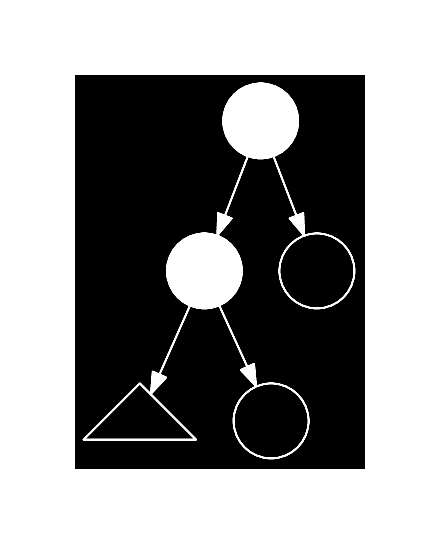
\includegraphics[scale=0.5]{figures/shape}

\end{columns}

\end{frame}

\begin{frame}[fragile]

\begin{codebox}
\Procname{$\proc{Ensure-Exhaustive}(c : C)$}
\li $P_{siblings} \gets \proc{Get-Siblings}(c)$
\li $C' \gets [c]$
\li \For $c'\in C$ \Do
\li $(P_{success},P_{fail}) \gets \proc{Match-Clause-To-Siblings}(c,P_s)$
\li \For $p\in P_{success}$ \Do
\li $c'' \gets \proc{Clone}(c')$
\li $\proc{Merge-Pattern}(c'',p)$
\li $C' \gets c' : C'$ \End
\li $P_{siblings} \gets P_{fail}$ \End
\li \Return $C'$
\end{codebox}

{\bf Invariants:}

\begin{itemize}

\item \bi $P_{siblings}$ is always a list of siblings that wasn't matched by
any forthcoming clause.

\item \bi $P_{success}$ and $P_{fail}$ are always sibling lists.

\end{itemize}

\end{frame}
